\chapter{Implementation}
In this chapter we describe implementation of Giflang and provide insights into the decisions we made along the way. As Figure \ref{fig:chap4:overview} shows,
the project consists of two major parts: an interpreter and a web IDE. These two components can be found in the \texttt{interpreter/} and the \texttt{frontend/}
folders, respectively. The Figure \ref{fig:chap4:overview} also outlines the API of the interpreter that allows the web IDE to execute user's programs.
This API is further discussed in subsection /TODO/
\begin{figure}[!hbt]
    \centering
    \label{fig:chap4:overview}
    \tikzset{every picture/.style={line width=0.75pt}} %set default line width to 0.75pt        
    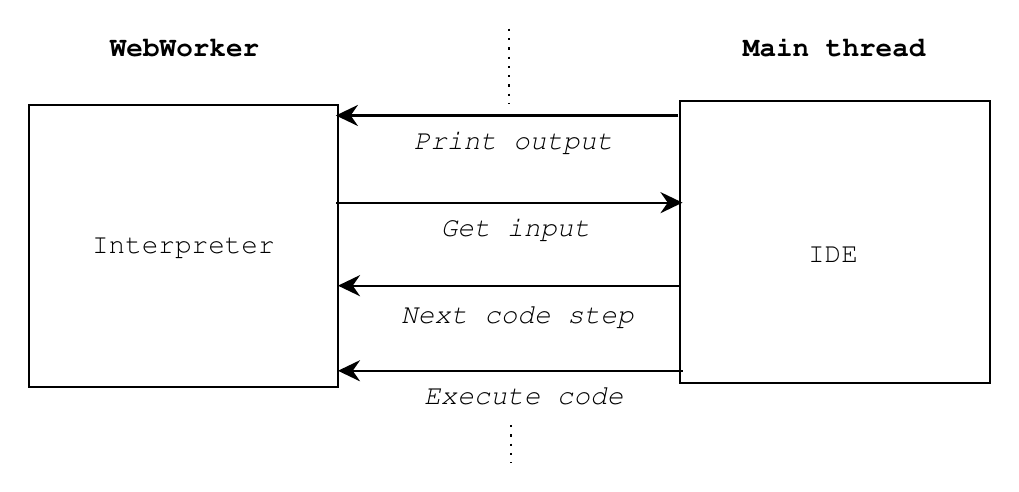
\begin{tikzpicture}[x=0.75pt,y=0.75pt,yscale=-1,xscale=1]
    \draw   (37.5,92) -- (186.5,92) -- (186.5,228) -- (37.5,228) -- cycle ;
    \draw    (352.5,220) -- (189.5,220) ;
    \draw [shift={(186.5,220)}, rotate = 360] [fill={rgb, 255:red, 0; green, 0; blue, 0 }  ][line width=0.08]  [draw opacity=0] (10.72,-5.15) -- (0,0) -- (10.72,5.15) -- (7.12,0) -- cycle    ;
    \draw    (351.5,179) -- (189.5,179) ;
    \draw [shift={(186.5,179)}, rotate = 360] [fill={rgb, 255:red, 0; green, 0; blue, 0 }  ][line width=0.08]  [draw opacity=0] (10.72,-5.15) -- (0,0) -- (10.72,5.15) -- (7.12,0) -- cycle    ;
    \draw    (349.5,139) -- (185.5,139) ;
    \draw [shift={(352.5,139)}, rotate = 180] [fill={rgb, 255:red, 0; green, 0; blue, 0 }  ][line width=0.08]  [draw opacity=0] (10.72,-5.15) -- (0,0) -- (10.72,5.15) -- (7.12,0) -- cycle    ;
    \draw    (350.5,97) -- (188.5,97) ;
    \draw [shift={(185.5,97)}, rotate = 360] [fill={rgb, 255:red, 0; green, 0; blue, 0 }  ][line width=0.08]  [draw opacity=0] (10.72,-5.15) -- (0,0) -- (10.72,5.15) -- (7.12,0) -- cycle    ;
    \draw  [dash pattern={on 0.84pt off 2.51pt}]  (269,55.2) -- (269,91.2) ;
    \draw  [dash pattern={on 0.84pt off 2.51pt}]  (270,246.2) -- (270,264.2) ;
    \draw   (351.5,90) -- (500.5,90) -- (500.5,226) -- (351.5,226) -- cycle ;
    \draw (425,164) node   [align=left] {{\fontfamily{pcr}\selectfont IDE}};
    \draw (112.02,161) node   [align=left] {{\fontfamily{pcr}\selectfont Interpreter}};
    \draw (112.6,64.4) node  [font=\normalsize] [align=left] {{\fontfamily{pcr}\selectfont \textbf{WebWorker}}};
    \draw (425.6,64.4) node  [font=\normalsize] [align=left] {{\fontfamily{pcr}\selectfont \textbf{Main thread}}};
    \draw (276.02,232) node   [align=left] {{\fontfamily{pcr}\selectfont \textit{Execute code}}};
    \draw (273.02,194) node   [align=left] {{\fontfamily{pcr}\selectfont \textit{Next code step}}};
    \draw (272.02,152) node   [align=left] {{\fontfamily{pcr}\selectfont \textit{Get input}}};
    \draw (271.02,110) node   [align=left] {{\fontfamily{pcr}\selectfont \textit{Print output}}};
    \end{tikzpicture}
    \caption{A high-level diagram of the implementation}
\end{figure}

\section{Interpreter}
Every interpreter first \emph{parses} a source code and then \emph{executes} the parsed tree (Fig \ref{fig:chap4:interpreter}). There is a room for a lot of optimizations along the way in order
to make the execution as fast as possible. However, we do not incorporate any optimizations into the interpreter and only execute the parsed tree node by node.

\begin{figure}[!hbt]
    \centering
    \label{fig:chap4:interpreter}
    \tikzset{every picture/.style={line width=0.75pt}} %set default line width to 0.75pt        

    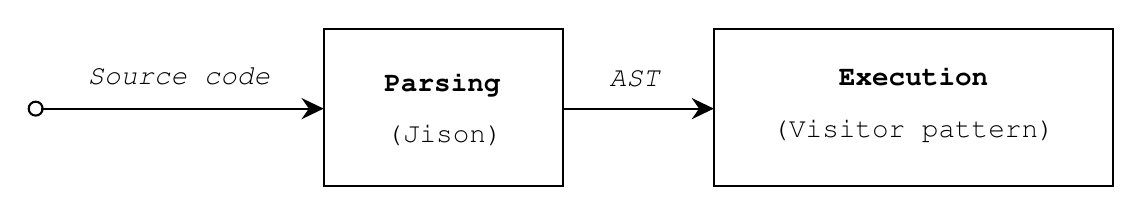
\begin{tikzpicture}[x=0.75pt,y=0.75pt,yscale=-1,xscale=1]
    %uncomment if require: \path (0,622); %set diagram left start at 0, and has height of 622

    %Shape: Rectangle [id:dp28122229657926034] 
    \draw   (226.5,34) -- (341.5,34) -- (341.5,110) -- (226.5,110) -- cycle ;
    %Straight Lines [id:da9888936135364137] 
    \draw    (411.25,72.5) -- (341.5,72.5) ;

    \draw [shift={(414.25,72.5)}, rotate = 180] [fill={rgb, 255:red, 0; green, 0; blue, 0 }  ][line width=0.08]  [draw opacity=0] (10.72,-5.15) -- (0,0) -- (10.72,5.15) -- (7.12,0) -- cycle    ;
    %Shape: Rectangle [id:dp7793277711435098] 
    \draw   (414.5,34) -- (606.5,34) -- (606.5,110) -- (414.5,110) -- cycle ;
    %Straight Lines [id:da7940866772557511] 
    \draw    (223.25,72.5) -- (89.85,72.5) ;
    \draw [shift={(87.5,72.5)}, rotate = 180] [color={rgb, 255:red, 0; green, 0; blue, 0 }  ][line width=0.75]      (0, 0) circle [x radius= 3.35, y radius= 3.35]   ;
    \draw [shift={(226.25,72.5)}, rotate = 180] [fill={rgb, 255:red, 0; green, 0; blue, 0 }  ][line width=0.08]  [draw opacity=0] (10.72,-5.15) -- (0,0) -- (10.72,5.15) -- (7.12,0) -- cycle    ;

    % Text Node
    \draw (283.5,61) node   [align=left] {{\fontfamily{pcr}\selectfont \textbf{Parsing}}};
    % Text Node
    \draw (510.5,57) node   [align=left] {{\fontfamily{pcr}\selectfont \textbf{Execution}}};
    % Text Node
    \draw (376.5,58) node   [align=left] {{\fontfamily{pcr}\selectfont \textit{AST}}};
    % Text Node
    \draw (284.5,85) node   [align=left] {{\fontfamily{pcr}\selectfont (Jison)}};
    % Text Node
    \draw (510.5,83) node   [align=left] {{\fontfamily{pcr}\selectfont (Visitor pattern)}};
    % Text Node
    \draw (156.5,57) node   [align=left] {{\fontfamily{pcr}\selectfont \textit{Source code}}};
    \end{tikzpicture}
    \caption{A diagram of Giflang interpreter}
\end{figure}

\subsection{Parsing}
Parser is an interpreter component that checks whether the input source conforms to the rules of the formal grammar of a language. Additionally, parsers help
building an AST from the source code. In the very beginning of this thesis we briefly explained what grammar rules and AST is (see Fig \ref{fig:chap1:tokens_and_grammar})

Parsers usually consist of two separate parts: \emph{lexing} or \emph{tokenization} and \emph{parsing}. A lexer splits input text into \emph{tokens}.
For example it can split an input \texttt{'4 + size'} into following tokens:
\begin{code}
// Sample tokens for an input '4 + size'
[{ "Type": "NUMBER", "Text": "4" },
 { "Type": "OPERATOR", "Text": "+" },
 { "Type": "IDENTIFIER", "Text": "size" }]
\end{code}

Grammar rules are then defined in terms of tokens, for example:
\begin{figure}
    \begin{code}
    expression -> factor OPERATOR expression
    expression -> factor
    factor -> IDENTIFIER
    factor -> NUMBER
    \end{code}
    \caption{An example of a grammar definition}
    \label{fig:chap4:grammar}
\end{figure}

The grammar above defines a language consisting of expressions that can contain numbers and identifiers. It is very minimal as it does not account
for operator precedence or parenthesis. Lowercase words are \emph{nonterminals} and capitalized words are \emph{terminals}. Terminal symbols are elementary
symbols and can not be replaced by other terminals or nonterminals. Nonterminals can appear on the left side of productions and they are replaced by groups
of terminal symbols according to the production rules.

In order to parse a grammar like the one above, we can either create our own parser or use \emph{a parser generator}. We will briefly describe both options.

\subsubsection*{Recursive-descent parser}
A recursive-descent parser is a method of creating a parser from mutually recursive procedures where each procedure implements one of the nonterminals
of the grammar. We mention recursive-descent parsers here because it is very easy to create them. To give us a better idea of what it means to create
a function for each nonterminal, we created a parser for the grammar from Figure \ref{fig:chap4:grammar}

\begin{code}
def accept(token):
    if curToken() == token:
        nextToken()
        return 1
    return 0

def expect(token):
    if accept(token):
        return 1
    raise Exception("expect: unexpected token")

def factor():
    if accept('IDENTIFIER'):
        # Action
        pass
    elif accept('NUMBER'):
        # Action
        pass 
    else:
        raise Exception("factor: syntax error")

def expression():
    factor()
    if accept('OPERATOR'):
        expression()
        # Action
\end{code}
\subsubsection*{Jison}

\subsection{Object model}
Everything is an object...

\subsection{Environment state}

\subsection{Auxiliary letters}

\subsection{Code stepping (debugger)}

\subsection{Additive input}

\subsection{API}

\section{IDE}

\subsection{Choosing image format}

\subsection{State management (Redux)}

\subsection{Layout}